%Fiquemos com Deus e Nossa Senhora!
%Sao Jose de Cupertino rogai por nos!!
% ### Uses XeLaTeX ### %
% ### Needs beamer-master ### %
\documentclass[aspectratio=169]{beamer} %. Aspect Ratio 16:9

\usetheme{AI2} % beamerthemeSprace.sty
\usepackage[portuguese]{babel}
\usepackage[utf8]{inputenc}
\usepackage[T1]{fontenc}
\usepackage{ragged2e}

\DeclareMathOperator*{\argmin}{arg\,min}

% DATA FOR FOOTER
\date{2021}
\title{- Regressão Logística}
\author{João Paulo Papa}
\institute{Advanced Institute for Artificial Intelligence (AI2)}

\begin{document}
% ####################################
% FIRST SLIDE 						:: \SliTit{This is the Title of the Talk}{A. B. Name}{Sprace}
% SUB-TITLE SLIDE 					:: \SliSubTit{<title>}{<explanation}
% SUB-SUB-TITLE SLIDE				:: \SliSubSubTit{<title>}{<explanation}
% SLIDE WITH TITLE 					:: \SliT{Title}{Content}
% SLIDE NO TITLE 						:: \Sli{Content} 
% SLIDE DOUBLE COLUMN WITH TITLE 	:: \SliDT{Title}{First Column}{Second Column}
% SLIDE DOUBLE COLUMN NO TITLE 		:: \SliD{First Column}{Second Column}
% SLIDE ADVANCED WITH TITLE 			:: \SliAdvT{Title}{Content}
% SLIDE ADVANCED NO TITLE 			:: \SliAdv{Content}
% SLIDE ADVANCED DOUBLE WITH TITLE 	:: \SliAdvDT{Title}{First Column}{Second Column}
% SLIDE ADVANCED DOUBLE NO TITLE 	:: \SliAdvD{First Column}{Second Column}
% SLIDE BLACK						:: \Black{ <Content> }
% SLIDE WHITE						:: \White{ <Content> }
% ITEMIZATION 						:: \begin{itemize}  \iOn{First} \iTw {Second} \iTh{Third} \end{itemize}
% COMMENT TEXT				 		:: \note{<comment>}
% SECTION 							:: \secx{Section} | \secxx{Sub-Section}
% BOLD SPRACE COLOR				:: \bfs{<text>}
% TABLE OF CONTENT					:: \tocitem{<title>}{<content>}
% LEFT ALIGN EQUATION				:: \begin{flalign*}  & <equation> &   \end{flalign*}
% CENTER ALIGN EQUATION	S			:: \begin{gather*} <equations>  \end{gather*}
% SLASH								:: \slashed{<>}
% BAR								:: \barr{<letter>} instead of \bar{<letter>}
% THEREFORE						:: use \portanto (larger and bold}
% 2 or 3 MATH SYMBOLS				:: \overset{<up>}{<down>} &  \underset{<below>}{\overset{<above>}{<middle>}}  
% INSERT TEXT IN FORMULA			:: \ins{<text>}
% EXERCISE							:: \exe{<exercise #>}{<exercise text>}
% SUGGESTED READING BOX			:: \sug{<references>}
% CITATION							:: \cittex{<citation>}
% CITATION DOUBLE COLUMN 			:: \cittexD{<citation>}
% TEXT POSITION						:: \texpos{<Xcm>}{<Ycm>}{<text>} origin = center of slide : x right | y down
% REFERENCE AT BOTTOM  S/D SLIDE		:: \refbotS{<reference>} \refbotD{<reference>}
% HIDDEN SLIDE						:: \hid
% COLOR BOX 						:: \blu{blue} + \red{rec} + \yel{yellow} + \gre{green} + \bege{beige}
% FRAME 							:: \fra{sprace} \frab{blue} \frar{red} + \fray{yellow} + \frag{green}		
% FIGURE 							:: \img{X}{Y}{<scale>}{Figure.png} 
% FIGURE							:: \includegraphics[scale=<scale>]{Figures/.png}
% FIGURE DOUBLE SLIDE NO TITLE		::  \img{-4}{0.5}{<scale>}{Figure.png} % Image 1st half
%									::  \img{4}{0.5}{<scale>}{Figure.png} % Image 2nd half
% FIGURE DOUBLE SLIDE WITH TITLE		::  \img{-4}{0}{<scale>}{Figure.png} % Image 1st half
%									::  \img{4}{0}{<scale>}{Figure.png} % Image 2nd half
% INCLUDING SWF (Flash)				:: \usepackage{media9} and \includemedia >> USE ACROBAT <<
%%%%%%%%%%%%%%%%%%%%%%%%%%%%%%%%%%%%%%%%%%%%%%%%%%
% ###############################################################################
% FIRST SLIDE
\SliTit{Regressão Logística}{Advanced Institute for Artificial Intelligence -- AI2}{https://advancedinstitute.ai}
%%%%%%%%%%%%%%%%%%%%%%%%%%%%%%%%%%%%%%%%%%%%%%%%%%
% ###############################################################################
% SLIDE SUB-TITLE
%\SliSubTit{Sub-Title}{Description}{}
%%%%%%%%%%%%%%%%%%%%%%%%%%%%%%%%%%%%%%%%%%%%%%%%%%
% ###############################################################################
%\SliSubSubTit{Sub-Sub-Title}{Description}
 %%%%%%%%%%%%%%%%%%%%%%%%%%%%%%%%%%%%%%%%%%%%%%%%%%


\SliT{Introdução}{
\secx{Regressão Logística}

\justifying Existem problemas para os quais desejamos estimar a \textbf{classe} (rótulo) de uma determinada amostra com base no seu conjunto de dados de entrada, isto é, as \textbf{características} do seu problema.

\justifying Problemas de classificação são similares aos de regressão pois desejamos aprender uma função que, dada uma entrada, estime um valor de saída. A diferença é que nossa saída será mapeada para uma \textbf{probabilidade} (\emph{soft classification}) ou \textbf{rótulo} (\emph{hard classification}) da amostra.

\justifying A técnica de Regressão Logística é uma das mais utilizadas na literatura, principalmente por ser simples e dar bons resultados em diversas situações. Ela tem esse nome pelo fato de estimar a probabilidade de uma dada amostra pertencer à uma classe em específico. Portanto, é uma técnica de classificação do tipo \emph{soft}.
}

\Sli{
\justify \underline{Definição do problema:} seja um conjunto de dados ${\cal X}= \{(\boldsymbol{x}_1,y_1),(\boldsymbol{x}_2,y_2),\ldots,(\boldsymbol{x}_z,y_z)\}$ tal que $\boldsymbol{x}_i\in\mathbb{R}^{n+1}$ corresponde ao dado de entrada e $y_i\in[0,1]$ denota o seu respectivo valor de saída. Temos, ainda, que ${\cal X}$ pode ser \textbf{particionado} da seguinte forma: ${\cal X} = {\cal X}^1\cup {\cal X}^2$, em que ${\cal X}^1$ e ${\cal X}^2$ denotam os conjuntos de dados de \textbf{treinamento} e \textbf{teste}, respectivamente. Nosso objetivo é, dado o conjunto de treinamento, aprender uma função $h:\mathbb{R}\rightarrow[0,1]$ que consiga estimar a probabilidade de uma amostra pertencer à uma dada classe. Por que usar uma função logística (sigmoide)?
}

\Sli{
A Função Logística possui algumas propriedades interessantes com a seguinte formulação:

\begin{equation}
	g(a)=\frac{1}{1+e^{-a}},
\end{equation}
tal que $g(a)\in[0,1]$.
\begin{center}
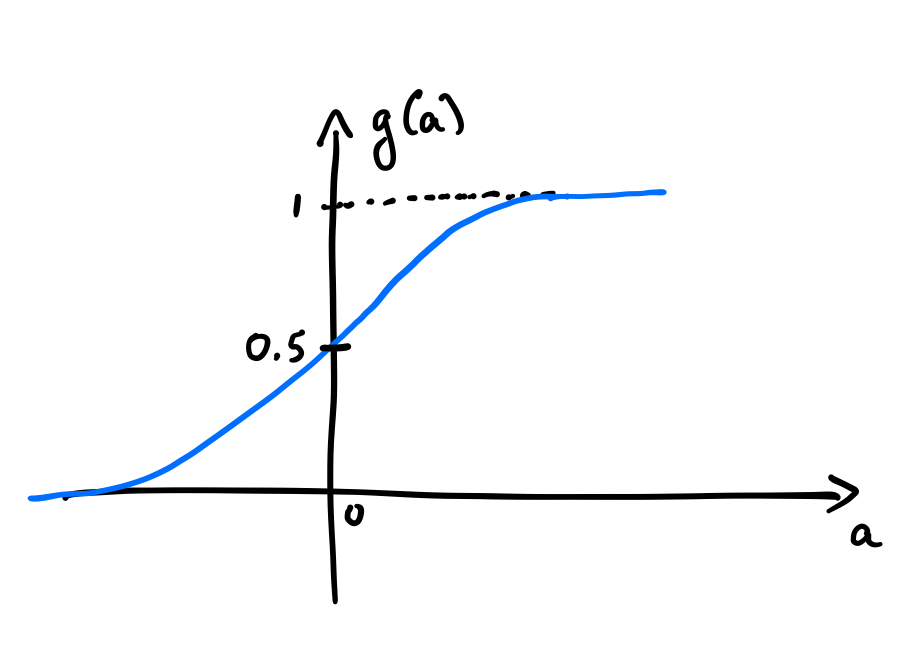
\includegraphics[scale=0.17]{./figs/Regressao_Logistica_Fig1.png}\hspace{1cm}
\end{center}
}

\Sli{
Como funciona o Regressor Logístico? Dado que queremos obter uma saída $h_{\boldsymbol{w}}(\boldsymbol{x})\in[0,1]$, basta modificarmos nossa entrada na Equação 1 como segue:

\begin{align}\nonumber
	h_{\boldsymbol{w}}(\boldsymbol{x}) &= g(\boldsymbol{w}^T\boldsymbol{x})\\
	&= \frac{1}{1+e^{-\boldsymbol{w}^T\boldsymbol{x}}}.
\end{align}

\begin{minipage}{0.49\textwidth}
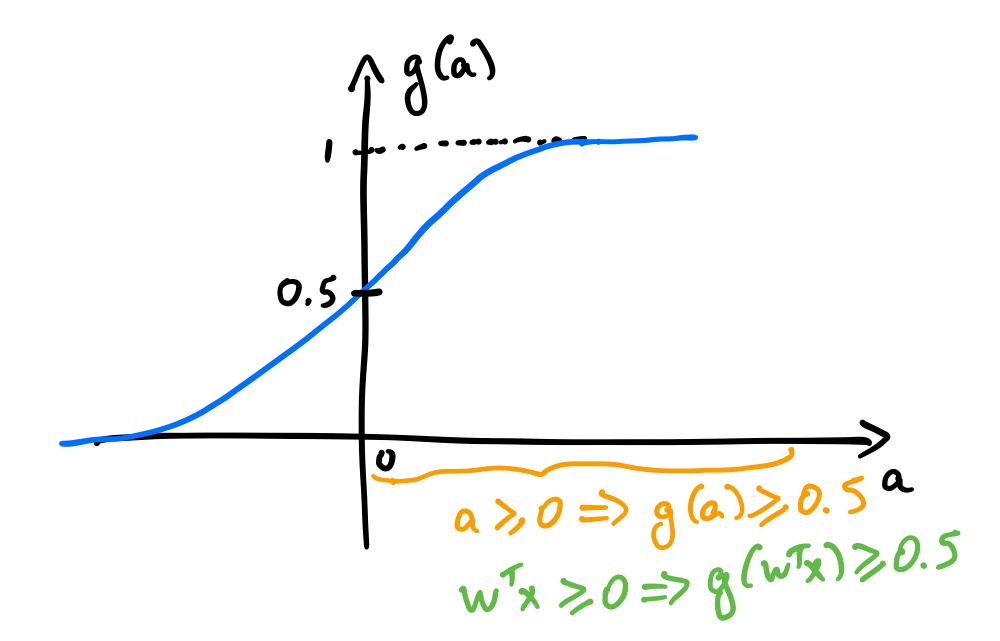
\includegraphics[scale=0.17]{./figs/Regressao_Logistica_Fig2.png}
\end{minipage}%%% to prevent a space
\begin{minipage}{0.37\textwidth}
Na prática, queremos que $h_{\boldsymbol{w}}(\boldsymbol{x})\geq 0.5$ quando $\boldsymbol{w}^T\boldsymbol{x}\geq 0$. De maneira análoga, temos que $h_{\boldsymbol{w}}(\boldsymbol{x})< 0.5$ quando $\boldsymbol{w}^T\boldsymbol{x}< 0$.
\null
\par\xdef\tpd{\the\prevdepth}
\end{minipage}
}	

\Sli{
Suponha que tenhamos a seguinte situação.
}

\end{document}